
\chapter{Experimentelle Untersuchungen}


Im vorliegenden Kapitel werden die Bestandteile und die Herstellung der Bauteilversuche beschrieben.



\section{Allgemeine Beschreibung der Bauteilversuche}


Die Schichtenabfolge und die Schichtenhöhe bzw. die Bauteilhöhe war bei allen Versuchen unverändert. In Abbildung \ref{sandwichaufbau} ist der Sandwichaubau  mit den verwendeten Dicken dargestellt.

\begin{figure}[h]
\begin{center}
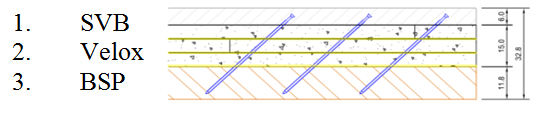
\includegraphics[scale =0.9]{Aufbau/bauteile/sandwich.png}
\caption{Sandwichaufbau}
\label{sandwichaufbau}
\end{center}
\end{figure}



\subsection{Verwendete Bauteilkomponenten}
\subsubsection{Selbstverdichtender Beton, SVB}

Selbstverdichtender Beton ist ein besonders fließfähiger Beton, der sich selbst entlüftet und eine ebene Oberfläche bildet. Durch die Fließfähigkeit ist ein besonders guter Verbund mit dem porösem Werkstoff Holzbeton (Velox) gewährleistet. Die Betonschicht wurde auf eine minimale Dicke von \unit[6]{cm} reduziert. Das Limit ergibt sich aus der Verankerungslänge der Schrauben (\unit[4]{cm}) zuzüglich einer Betondeckung von \unit[2]{cm}. Die Betonrezeptur hat Kirchmayer [] ausgearbeitet.


\begin{figure}[h]
\begin{center}
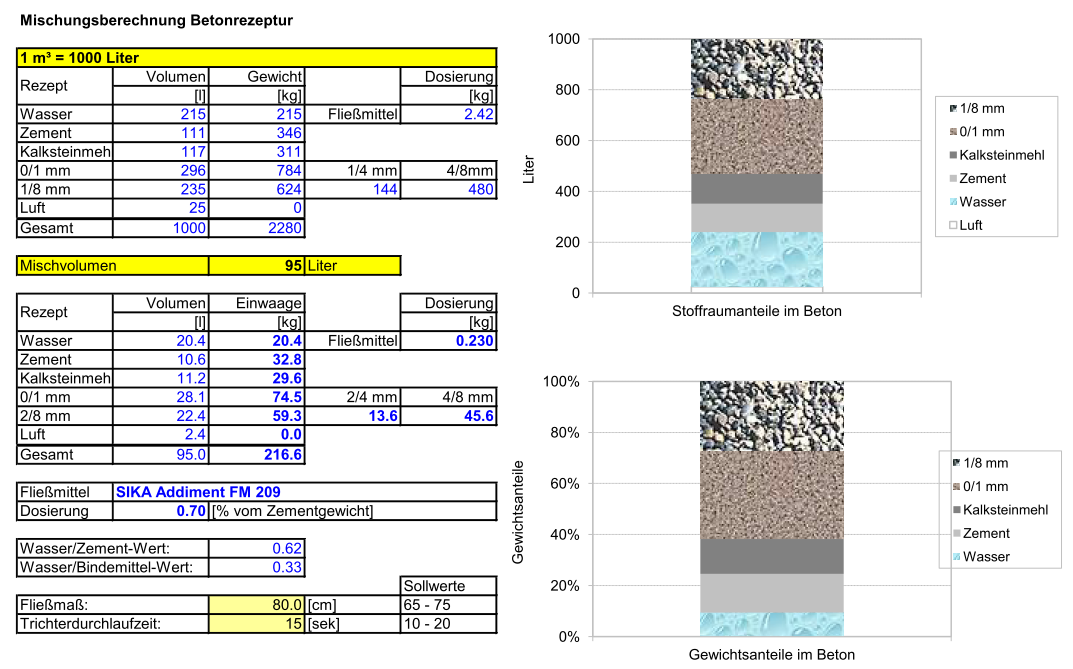
\includegraphics[scale =1.1]{Aufbau/bauteile/Beton-Mischrezeptur.png}
\caption{Beton-Mischrezeptur [2], mit Okamurarechner}
\label{Beton-Mischrezeptur}
\end{center}
\end{figure}


\subsubsection{Holzspanbeton/ Holzleichtbeton}

Holzspanbeton besteht aus den Komponenten Zement, Sägespänen, Wasser, Additiven und Zuschlagstoffen. Die Auswahl des Materials geht auf die Vorversuche von Kirchmayer bzw. Schernberger zurück. 
Die Abmessungen der Holzbetonschicht ergab sich aus einem Vielfachen der Dicke der Velox-Platten (\unit[50]{mm}) und aus Vorberechnungen mit den FEM-Programm        "`Sofistik"'. Die Veloxplatte ist ein Industrieprodukt, das ausführlich in der Ausarbeitung von Kirchmayer beschrieben wird.


\begin{figure}[h]
\begin{center}
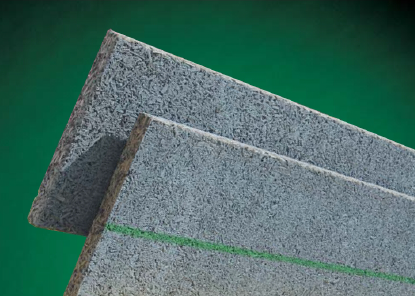
\includegraphics[scale =0.7]{Aufbau/bauteile/velox.png}
\caption{Holzspanplatte WS 50 der Firma Velox}
\label{velox}
\end{center}
\end{figure}

\subsubsection{Brettsperrholz, BSP}

Die Brettsperrholzplatte ist ein flächiges Holzprodukt aus mindestens drei rechtwinkelig zueinander verleimten Schichten. BSP wird im Holzmassivbau eingesetzt und kann mit großen Abmessungen hergestellt werden. Es wurde auch schon in den Vorversuchen von Kirchmayer angewendet. Die Vorteile hat ebenfalls  Kirchmayer [] schon ausgearbeitet.

Es wurde für alle Bauteilversuche das Produkt BSP 118 3s DL ind. verwendet. In Abbildung \ref{clt} ist ein Beispielbild einer fünf-schichtigen BSP-Platte dargestellt.

\begin{figure}[h]
\begin{center}
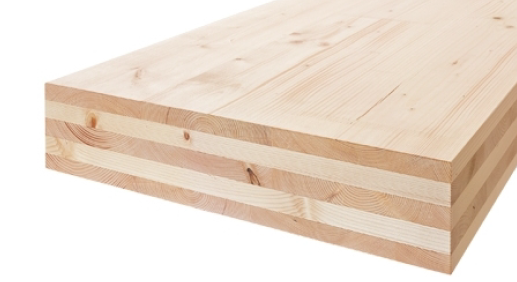
\includegraphics[scale =0.7]{Aufbau/bauteile/clt.png}
\caption{fünfschichtige Brettsperrholzplatte (BSP der Fa. Mayr-Melnhof)}
\label{clt}
\end{center}
\end{figure}

\subsubsection{Verbindungsmittel}

Um einen kraftschlüssigen Verbund der einzelnen Bauelemente herstellen zu können, kamen verschiedene Verbindungsmittel zur Anwendung. Aus den Vorversuchen von Kirchmayer ist hervorgegangen, dass die besten Verbundergebnisse durch Schrauben und Kleber  erzielt worden sind. Dieser Ansatz wurde weiter verfolgt.




\begin{itemize}
\item Schrauben
\newline
Die verwendeten Schrauben sind durch die Versuche ( Siehe Kapitel\,2) ausgewählt worden.
\newline
\begin{itemize}
\item SFS Intec WR-T-9x400
\end{itemize}

\item Kleber

Die angeführten Kleber sind im Kapitel 2 beschrieben.
\newline

\begin{itemize}
\item Sikadur-31 AUT Normal
\item SikaTop-109 ElastoCem 
\item Sikatop-107 Seal
\end{itemize}

\end{itemize}

\subsection{Herstellung des Sandwichaufbaus}
Der Zweikomponenten-Kleber wurde mit dem Mischverhältnis, das vom Hersteller angegeben wird, abgemischt. Die erste Kleberschicht wurde auf die BSP-Platte aufgetragen. Das Auftragen erfolgte mit einer  \unit[8]{mm} Zahnspachtel. Für die Verarbeitungszeit des Klebers war laut Datenblatt \unit[45]{min} Topfzeit vorgegeben. Auf die Kleberschicht wurden die Velox-Platten aufgelegt. Dieser Schritt wurde drei mal wiederholt. 

\begin{figure}[h!]
	\begin{minipage}[h]{7cm}	
	 	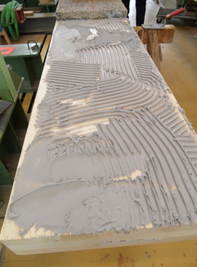
\includegraphics[width=7cm]{Aufbau/herstellung/kleberauftrag.png}
		\caption{Kleberauftrag auf die BSP-Platte}
		\label{kleberauftrag}
	\end{minipage}
		\hfill
	\begin{minipage}[h]{7cm}
		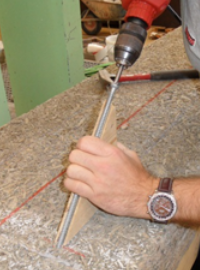
\includegraphics[width=7cm]{Aufbau/herstellung/einschrauben.png}
		\caption{Einschrauben der Schrauben}
		\label{einschrauben}
	\end{minipage}
\end{figure}




Im nächsten Schritt wurde das Bohrmuster auf der obersten Velox-Platte aufgezeichnet. Die Schrauben wurden mit einem Hilfswinkel (Holzstück) und einem Hammer angesetzt um den Einschraubwinkel   (\unit[45]{$^{\circ}$}) einzuhalten. Die Schrauben wurden anschließend ohne Vorbohren mit einer Bohrmaschine in den Bauteil eingebohrt, bis die Schrauben nur noch \unit[4]{cm} aus der oberen Velox-Schicht herausstanden. 
	

Der letzte Schritt vor dem Betonieren war das Anbringen der Schalung. Es wurden Schalungsbretter auf eine Höhe von \unit[20]{cm} zugeschnitten. Die Schalung wurde mit einem Überstand von \unit[6]{cm} über der letzten Veloxschicht angebracht. Damit man den Überstand allseitig gleich hält, wurden zwei Holzstücke mit den geforderten \unit[6]{cm} gefertigt. Somit hatte sich das Einrichten der Bretter einfach gestaltet.  Die Bretter wurden an die Velox-Schicht angeschraubt .


Abschließend wurde der Beton hergestellt. Die einzelnen Bestandteile wurden nach der Betonrezeptur [Abbildung: \ref{Beton-Mischrezeptur}] exakt eingewogen und mit einem Zwangsmischer vermischt. Der Beton wurde von Hand aufgebracht. Zum Schluss wurde der Beton mit einer Latte abgezogen und mit einem Schwert geglättet.


	



\begin{figure}[h!]
\begin{minipage}[h]{7cm}	
	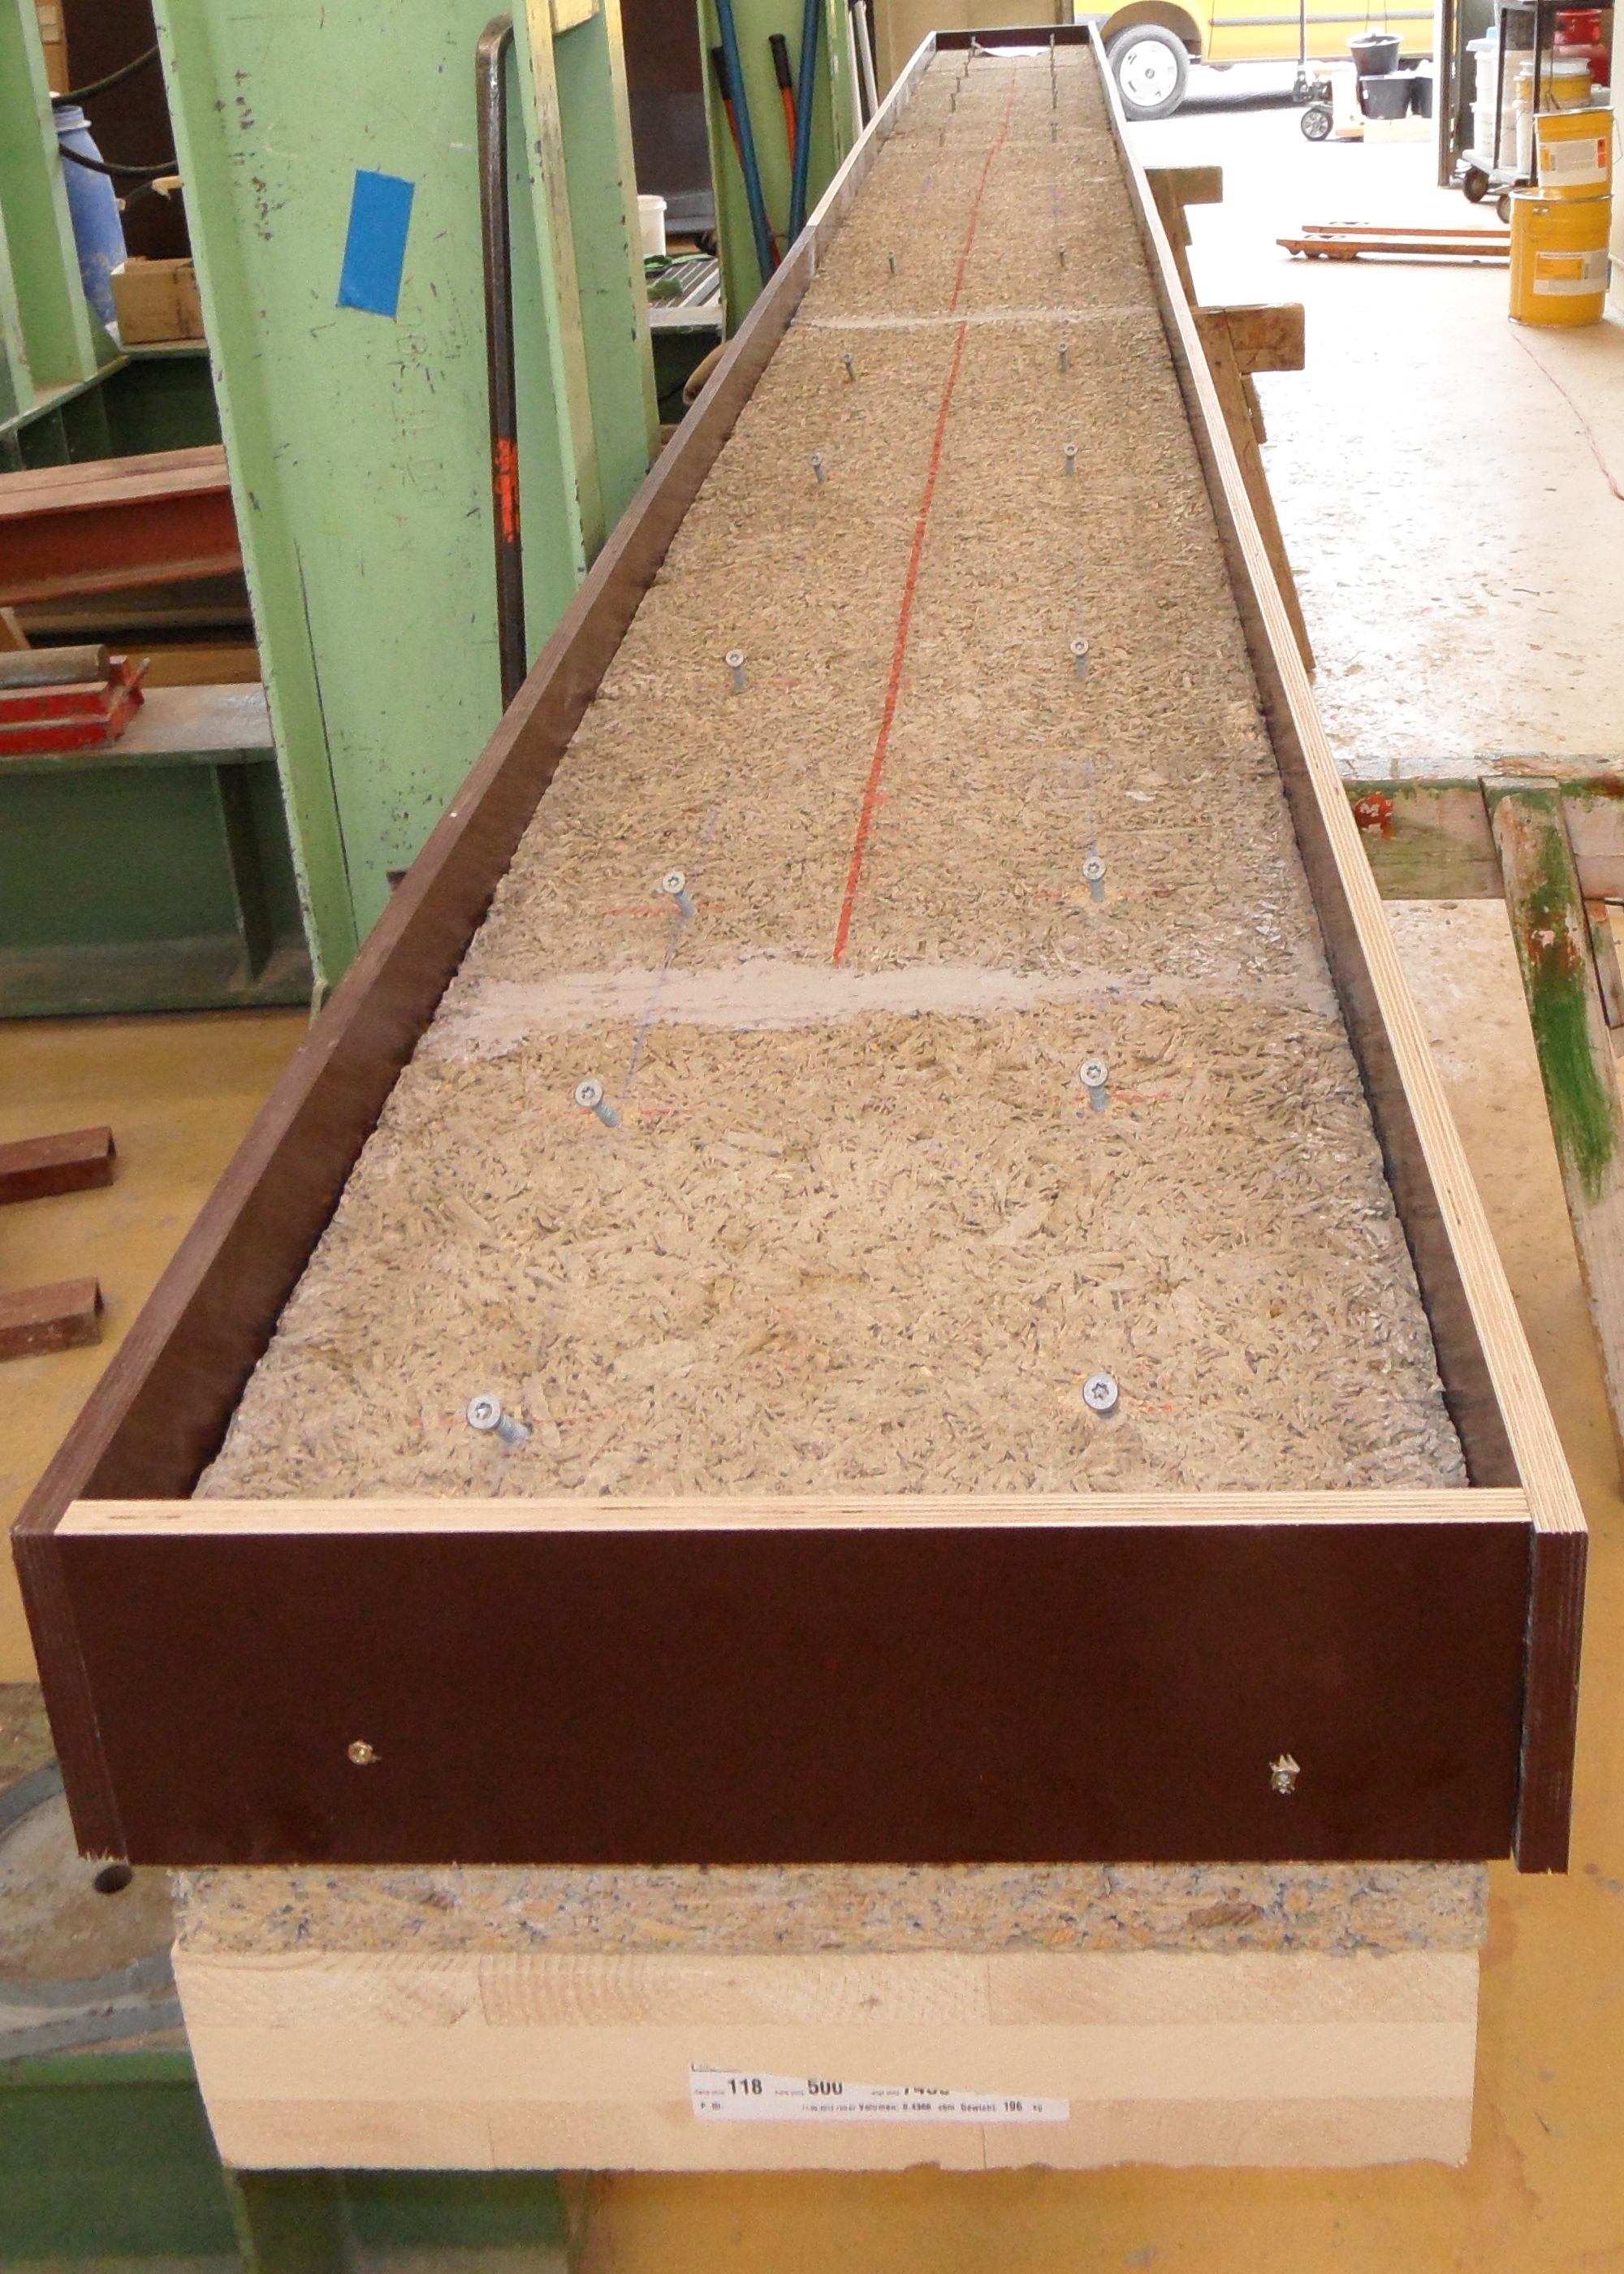
\includegraphics[width=7cm]{Aufbau/herstellung/einschalen.png}
	\caption{Befestigung der Schalung am Velox}
	\label{einschalen}
	
\end{minipage}
\hfill
\begin{minipage}[h]{7cm}
	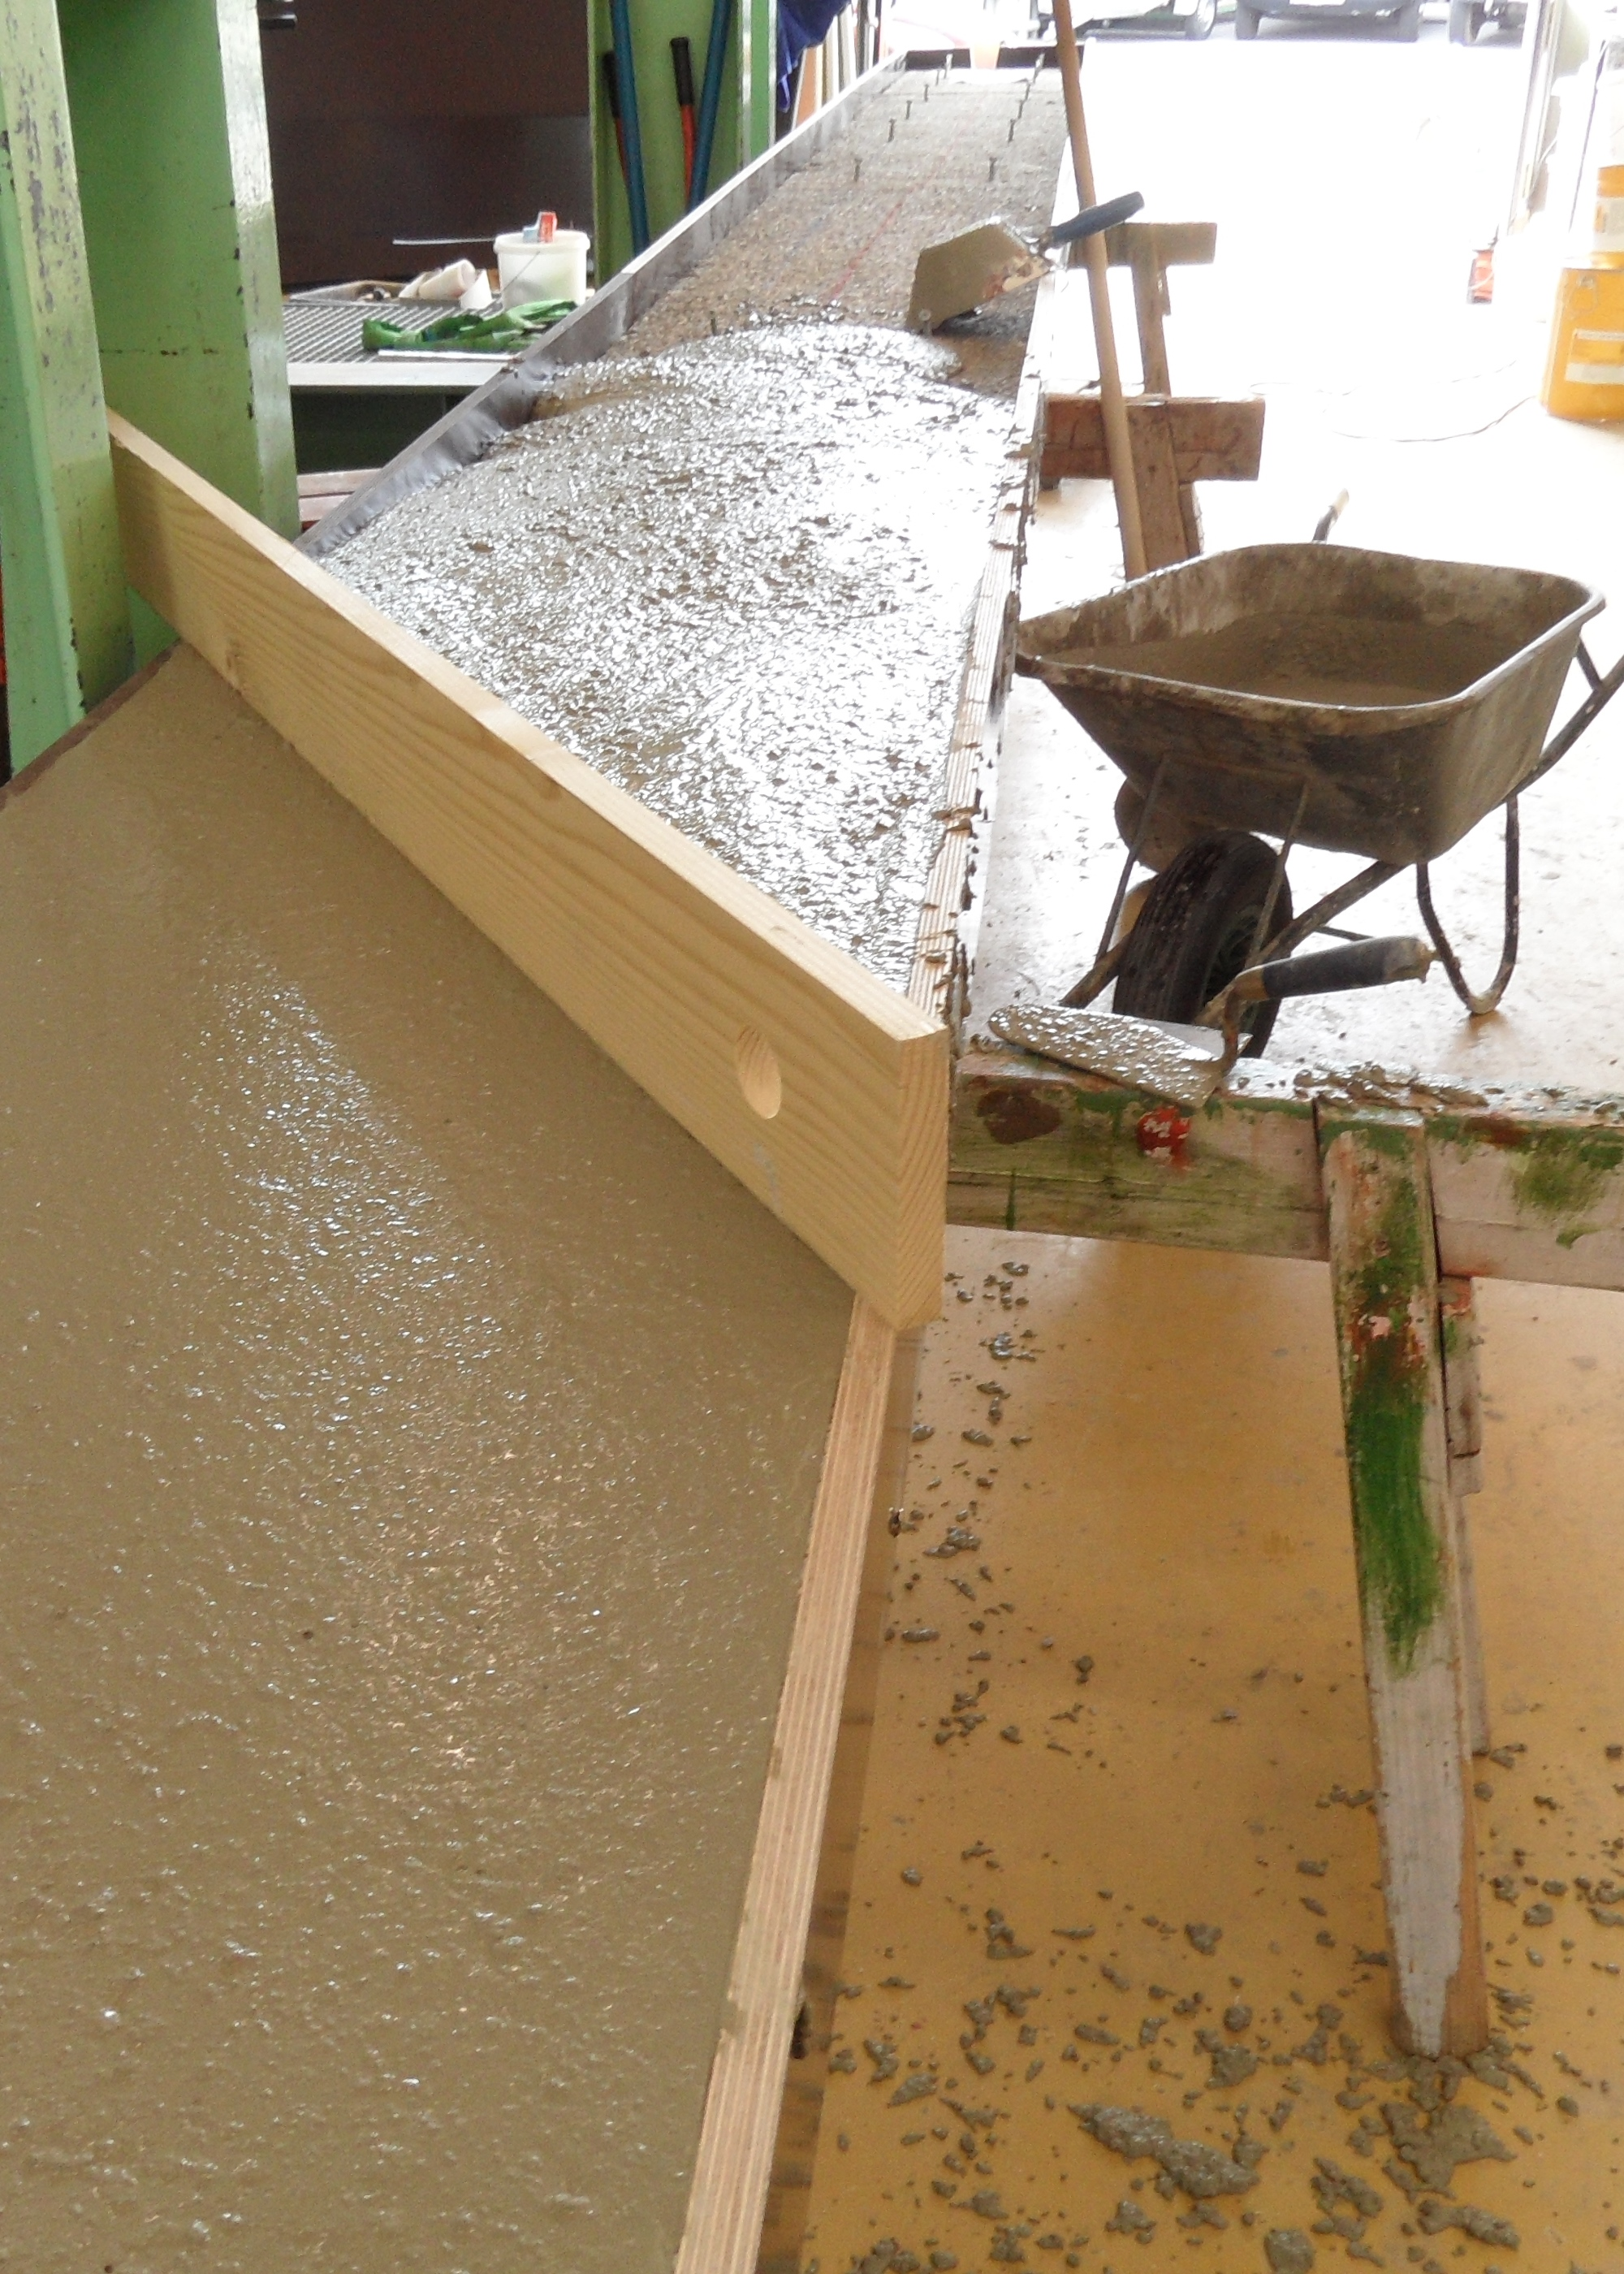
\includegraphics[width=7cm]{Aufbau/herstellung/betonieren.png}
	\caption{Einbrinden und Abziehen des SVB}
	\label{betonieren}
\end{minipage}
\end{figure}

